\section{Aufbau von M$^2$etis}
\label{chap:aufbau_metis}

Dieser Abschnitt erläutert den Aufbau von \ac{m2etis}  und zeigt den Rahmen dieser Diplomarbeit auf. \ac{m2etis} ist ein Framework für \acp{mmve} und hat als Ziel, die Verteilung der verschiedenen Events eines Spieles zu optimieren. Dabei wird nicht der klassische Ansatz einer Client-Server-Kommunikation, sondern ein dezentraler Ansatz mit einem Publish/Subscribe-System auf einem \ac{p2p}-Netzwerk, gewählt \cite{Fischer2010a}. Hierbei soll durch die unterschiedliche Behandlung einzelner Eventtypen die Verteilung dieser optimiert werden \cite{Fischer2010Event}.

\begin{figure}[htbp]
\centering
\resizebox{\textwidth}{!}{%
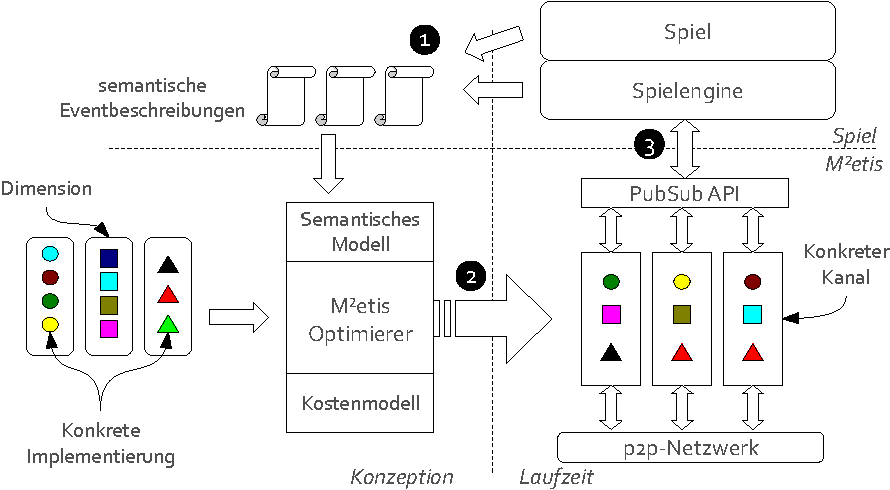
\includegraphics{grafics/metis_aufbau.pdf}}
\caption{Architekturübersicht von M$^2$etis}
\label{fig:metis_aufbau}
\end{figure}

\Fref{fig:metis_aufbau} zeigt die zeitliche Aufteilung des Systemes in \emph{Konzeption} und \emph{Laufzeit} sowie die Schnittpunkte von \ac{m2etis} mit dem \ac{mmve}. In der Grafik wird dieses durch ein \emph{Spiel} dargestellt.

Im ersten Schritt werden die im Spiel genutzten Eventtypen durch den Spielentwickler identifiziert und semantisch beschrieben. Im zweiten Schritt verarbeitet der \ac{m2etis} \emph{Optimierer} diese Beschreibungen unter Zuhilfenahme des \emph{semantischen Modells} und des \emph{Kostenmodells}. Für jeden Typ wird dabei ein optimierter \emph{Kanal} erzeugt, in dem die unterschiedlichen Implementierungen der in \cite{Fischer2010a} beschriebenen Dimensionen Anwendung finden.\\
Die optimierte Kanäle lassen sich zur Laufzeit (im 3. Schritt) über die Publish/Subscribe-API ansprechen und kommunizieren über das \ac{p2p}-Netzwerk. Zur Laufzeit soll das Spiel jedoch keine weiteren Implementierungsdetails der optimierten Kanäle kennen müssen um das System nutzen zu können.

Diese Arbeit beschränkt sich auf die Anbindung des gewählten \ac{p2p}-Netzwerk und die Konzeption des Publish/Subscribe-Systems. Damit das Framework frühzeitig einsetzbar ist und weitere Arbeiten darauf aufbauen können, werden zudem eine prototypische Implementierung des Publish/Subscribe-Systems erstellt. Die Konzeption des Kostenmodelles oder die Entwicklung des Optimierers würden den Rahmen dieser Diplomarbeit sprengen und bleiben nachfolgenden Arbeiten überlassen.
